\chapter{共識模組與系統架構}\label{se_5}

\section{共識模組}\label{se_5}
本章節介紹我們實作拜占庭容錯共識的架構與機制。,共識模組底下包含處理訊息的 message handler、同步訊息的 synchronizer、與三個主要做共識的模組, ConsensusManager、HeightManager 與 RoundManager。共識模組間的關西如下圖。

\begin{figure}[h]
\centering
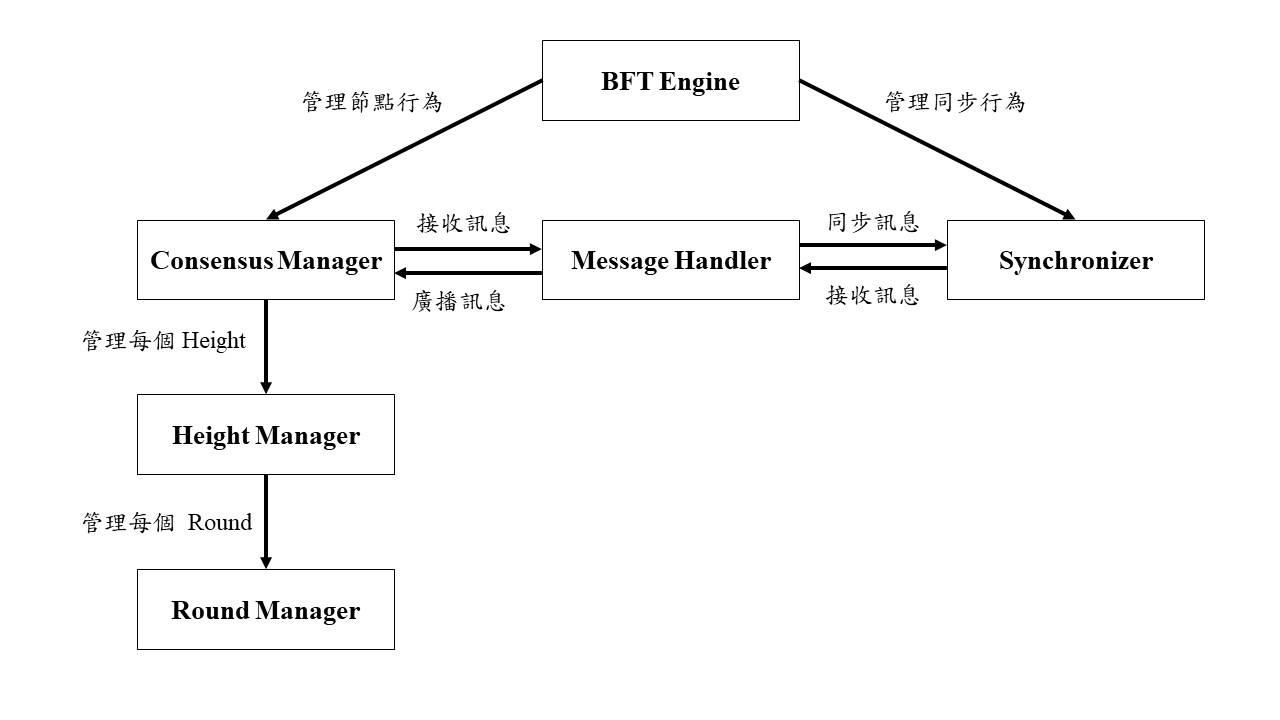
\includegraphics[scale=0.45]{images/5.jpg}
\caption{共識模組關係圖。}
\label{i:byz-latency}
\end{figure}


\subsection{Message Handler}\label{se_5} 
Message handler 主要負責接收與廣播共識之中需要的訊息,在接收到來自其他節 點的訊息時進行判斷是否交給 ConsensusManager,或是過濾掉重複接受的訊息。 
\subsection{Synchronizer}\label{se_5}
Synchronizer 主要目的為同步節點之間在做共識時需要的訊息,以及同步驗證區塊 所需要的訊息。節點可能因為網路延遲或是比較晚加入共識,少了前面的訊息而無法 執行共識,必須先與其他節點同步到最新狀態,所以需要 Synchronizer 進行這動作。  
\subsection{Consensus Manager}\label{se_5} 
主要功能是管理 HeightManager,以及區塊鏈本身與資料庫的各種資訊。 ConsensusManager 也負責處理與其他節點交換的各種資訊,再將收到的資訊向下 交給 HeightManager 處理,同時也要將需要廣播的資訊交給 message handler。
\subsection{Height Manager}\label{se_5}
此模組主要功能是處理某一個高度的共識,透過管理一或多個 RoundManager 與其他節點進行共識。
\subsection{Round Manager}\label{se_5}
每個高度會需要一到多個回合,HeightManager 會建立一到多個 RoundManager 來進行共識。RoundManager 會蒐集來自 HeightManager 的訊息,經過判斷後開始新的共識回合。




\section{系統架構}\label{se_5}  
FaS-BFT共識演算法相較於過去傳統三回合的共識演算法,能在網路傳輸穩定情況下,較快達成共識。我們的目標是測試FaS-BFT在數百個節點的私有鏈的效率,實驗將在AWS雲端伺服器上進行,為了達成這個目標,我們整合了許多自動化的開發套件來協助我們完成實驗。實驗系統架構主要如下圖所描述 

\begin{figure}[htbp]
\centering
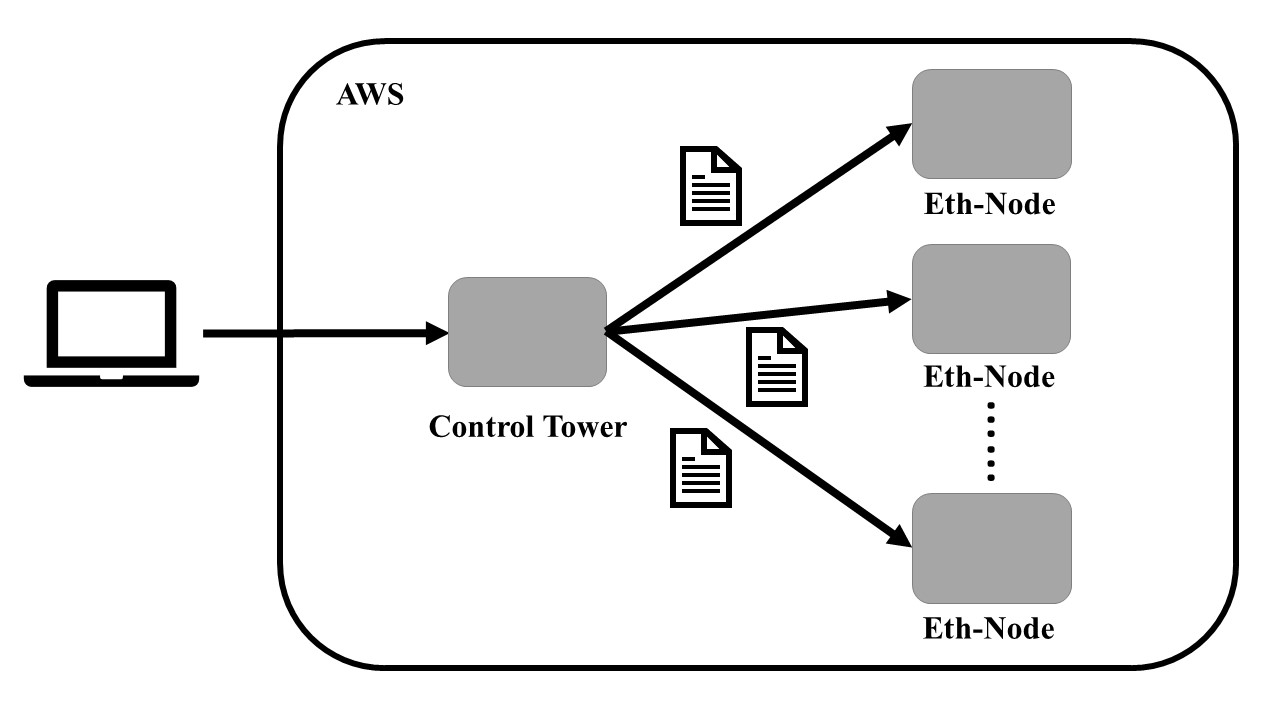
\includegraphics[scale=0.5]{images/51.jpg}
\caption{實驗系統架構圖。}
\label{i:byz-latency}
\end{figure}

該系統內含一個Control Tower,此台電腦類似實驗的中央控制中心,負責部署實驗環境到其他雲端機器上,並且收集其他機器所產生的實驗數據,該系統另包含數百個區塊鏈節點,這些節點運行FaS-BFT演算法來達成區塊鏈共識。自動化多節點實驗主要分為兩大步驟: (1)高效率部署雲端系統 (2)自動化搭建私有鏈
\subsection{高效率部署雲端系統}\label{se_5} 

\begin{itemize}%项目符号开始
\item [1)] Packer: 為了能夠快速將上百個區塊鏈節點環境建立起來,因此使用了Hashicorp Packer這套工具來打包 AWS的AMI (Amazon Machine Images),AMI 能幫助我們快速建立出環境一致的節點。
Packer的優點如下

\item 極快速的部署:因為已經把需要的套件及其他設定都放在映像檔中,所以馬上可用。

\item 跨平台且可攜性:Packer 可針對不同平台打包出完全相同的映像檔,可在本地、雲端等各種不同平台獲得相同的運行環境。

\item 較好的測試性:映像檔一打包完成就可進行各種測試。

\item [2)] Terraform: Terraform能夠快速將AWS環境架設起來,依照使用者所撰寫程式碼搭建出所描述的架構,Terraform好處是能徹底實現基礎架構即代碼IaC (Infrastructure as code),利用代碼來配置實驗環境,讓環境安全且方便管理。
Terraform的優點如下:
\item   將基礎架構使用語法進行描述,可讓建構計劃像一般程式碼一樣進行版本控管與追蹤。 

\item Terraform會自動分析本地端計劃與遠端是否一至,自動化修改從而避免許多可能的人為操作錯誤。

\subsection{自動化搭建私有鏈}\label{se_5} 

\item [1)] Ethereum Wallet api: 系統環境建立後我們將透過Control Tower 動態產生實驗所需節點資訊,在我們的 實驗裡透過Ethereum Wallet api 動態的自動產生與實驗所需節點數之節點資訊(Public key, Address等等)

\item [2)] Genesis.json: Genesis.json 裡定義了區塊鏈資訊(包含區塊大小,區塊ID, 鏈上節點初始以太幣),由於每次實驗所產生節點帳戶地址都不相同,故我們將Genesis.json 設計成自動化動態產生,以方便實驗進行。 

\item [3)]Eth-client: 在Eth-client裡我們會執行節點間相互交易,Eth-client幫助我們每秒產生數百筆交易,鏈上的節點才能打包這些交易成為候選區塊,故與Genesis.json 相同因每次實驗所產生節點帳戶地址都不相同,我們也將Eth-client設計成自動化動態產生。 

\item [4)] Ansible: Ansible能幫助我們定義系統上的角色,方便我們依照不同角色執行相對應動作(ex. Control Tower會推送執行檔給鏈上節點執行,鏈上節點將實驗結果回傳至Control Tower做實驗分析。)

Ansible的優點如下:

\item 輕量級套件,無需在客戶端安裝agent,更新時,只需在操作機上進行一次更新即可。

\item 可將任務寫成腳本批次執行。

\item 使用python編寫,維護更簡單 。
\end{itemize}